\documentclass[oneside,12pt]{book}
\usepackage[left=2cm,top=1cm,right=3cm,nofoot]{geometry}                % See geometry.pdf to learn the layout options. There are lots.
\geometry{a4paper}                   % ... or a4paper or a5paper or ... 
\usepackage{tabularx}
%\usepackage[latin1]{inputenc}
%fontspec,\usepackage{xltxtra,xunicode}
%\defaultfontfeatures{Mapping=tex-text}
%\usepackage[french]{babel}
\usepackage[utf8]{inputenc}
\usepackage[francais]{babel}
%\usepackage[cyr]{aeguill}
\usepackage{listings}
\usepackage{color}
\usepackage{graphicx}
\usepackage[linktocpage]{hyperref}

\setlength{\parindent}{20pt}

\newcommand\don[6]{
\textbf{#1} \\
(#6) - #2
\begin{itemize}
\item{ \textbf{jet}: #3}
\item{ \textbf{Cout}: #4}
\item{ \textbf{Page}: #5}
\end{itemize}
\vspace{0.5cm}
}

\newcommand\roll[1]{
( Jet: \textbf{#1})
}
%%%%%%%%%%%%%%%%%%%%%%%%
% Definition des variables
%%%%%%%%%%%%%%%%%%%%%%%%
\newcommand{\Lynn}{\textbf{Étoile Rouge} }
\newcommand{\Jessica}{\textbf{Sagesse Tenace} }
\newcommand{\Luke}{\textbf{Cendre Griffe} }
\newcommand{\Peter}{\textbf{Hurle Mort} }
\newcommand{\Leonard}{\textbf{Sombre Bois} }

%% PNJ
\newcommand{\Monster}{\textbf{Monster Under The Bed} }
\newcommand{\BlackEclipse}{\textbf{Black Eclipse} }
\newcommand{\Tails}{\textbf{Tails} }

\newcommand{\Elisabeth}{\textbf{Elisabeth Lecoeur} }
\newcommand{\Thomas}{\textbf{Zi'ir} }

\newcommand{\Christopher}{\textbf{Christopher} }

%% Meutes
\newcommand{\Night}{\textbf{Night Howlers} }
\newcommand{\Sadness}{\textbf{Sadness Knives} }
\newcommand{\Hidden}{\textbf{Hidden Claws} }

\title{Promenons-nous dans les bois}
\author{Renaud "ObiWan" Guezennec}
\date{}

%\let\origdescription\description
%\renewenvironment{description}{
%  \setlength{\leftmargini}{0em}
%  \origdescription
%  \setlength{\itemindent}{1em}
%}


\begin{document}

\maketitle \clearpage
\tableofcontents \clearpage
\listoffigures \clearpage

\begin{flushleft}
    \chapter{Introduction}
    \section{Cadre du scénario}
    Ce scénario a été écrit pour la 71ième Nuit Tenebrae dont le thème était \textbf{l'enfance}. 
    
    Il a été joué dans divers événements. 
    \begin{itemize}
    \item 71ième Nuit Tenebrae, le 18/02/2012 : \href{http://www.tenebrae-mundis.com/les-nuits-tenebrae/teaser-de-la-71e-nuit-tenebrae}{Lien}, cinq joueurs
    \item Eclipse, Convention de JDR de La Lune Rousse de Rennes : \href{http://www.ascreb.org/clubs/jdr/convention/archives/eclipse10.php}{Lien}, deux parties, onze joueurs
    \item RRX, Convention de JDR de Polytechnique 2012, deux parties, dix joueurs. 
    \item Les Joutes Du Téméraires (2012), convention de JDR de Nancy, cinq joueurs, :-)
    \item Octogones, convention de JDR à Lyon, deux parties, dix Joueurs.
    \item Session privée, cinq joueurs, Aout 2012.
    \item Session privée, cinq joueurs, Février 2013.
    \end{itemize}
    
    Total de joueurs: cinquante et un.

        \section{L'univers de loup-garou: les déchus}
       Les loups-garous sont mi-humains mi-esprits loups. 
       Il y a très longtemps, à une époque que certains nomment la Pangée, 
       Père Loup faisait régner l'ordre et l’équilibre entre le monde physique et le monde des esprits.\\ 
       Conquise par son courage, Mère Lune tomba amoureuse de lui et prit forme humaine pour le séduire. 
       Elle donna naissance à neuf enfants (les Premiers-Nés). 
       De leur mère ils reçurent la faculté de changer de forme et de leur père la force et l'instinct de chasseur.\\ 
       Le passage des siècles vit la naissance de plusieurs générations de loups-garous, 
       dans lesquelles le pouvoir de Père-Loup se dilua. 
       Une partie de sa meute réalisa qu'il était trop faible pour les guider et lui proposa son aide, mais il la refusa. Alors ses enfants assassinèrent Père-Loup car il refusait de partager son fardeau avec le fruit de sa chair. Lorsqu’il reçut le coup mortel, son cri fut si puissant qu’il déchira le monde. Depuis lors, Hisile, le monde des esprits, s’est éloigné du monde physique.\\ Les esprits en veulent aux loups-garous (urathas) car ils ont anéanti leur paradis et sont parvenus à tuer Père-Loup alors qu’eux n’y étaient jamais arrivés. Mère-lune maudit ses propres enfants pour les punir de leur crime et les rendit vulnérables à l'argent, le métal le plus précieux à ses yeux.\\ 
       Au fil des siècles, elle allégea la malédiction de ceux de ses enfants qui reprirent la tâche de son bien-aimé. 
       Ces loups-garous là sont les gardiens de l’équilibre entre le monde des esprits et le monde physique.  \\
Une nuit éternelle règne sur le monde des esprits. 
À l’exception des humains, dont les émotions l’alimentent, chaque élément du monde physique y trouve son reflet. 
Les esprits peuvent être des concepts comme la violence, la jalousie ou l'appétit, ou bien être le reflet d’objets ou d’animaux, comme une porte ou un renard.\\ Les loups-garous sont les seuls êtres autorisés à passer d’un monde à l’autre.
\subsection{Les trucs cools d'être loup-garou}
\begin{itemize}
\item Les 5 formes 
\item Locus
\item Régénération
\item Tribus
\end{itemize}

\subsection{Les ennemis}
\begin{itemize}
\item Les esprits : leur but est de grandir le plus possible.
\item Les purs : ils refusèrent de prendre part à la mort de Père-Loup et qui refusent de maintenir l'équilibre.
\item Humains : ils ignorent votre existence. S’ils la découvrent, ils auront des intentions hostiles.
\end{itemize}


\subsection{Serment de la Lune}
\begin{itemize}
\item Les loups doivent chasser
\item Le peuple ne tue pas le peuple
\item Le faible honore le fort, Le fort respecte le faible.
\item Respecte ta proie
\item Le peuple doit vivre parmi les humains
\item Ne mange pas de chair humaine ou de loup
\item Le troupeau ne doit pas savoir
\end{itemize}

  
\section{Les meutes}
\subsection{La Meute PJ : Night howlers}
\Lynn : Lynn Ethwings :  institutrice (Cahalithe, Griffe de Sang) \\
\Peter : Peter Torhes : sherif (Elodothe, Seigneur des Tempêtes) \\
\Luke : Luke Hereford : agriculteur (Rahu, Maître du Fer)\\
\Leonard : Leonard J. Andrews : garde-chasse (Irraka, Chasseur des Ténèbres)\\
\Jessica : Jessica  Ethwings : vétérinaire (Ithaeur, Os de l'Ombre)\\

\subsection{La meute sympa mais pas trop : Sadness knives}
\label{sadnessknives}
\textbf{\BlackEclipse} : Floria Centerfold (Alpha, Rahu, Chasseur des Ténèbres)\\
\textbf{Red Fangs} : David McClurgan  (Irraka, Chasseur des Ténèbres)\\
\textbf{Vicious Pain} : Helen Hallister (Cahalithe, Griffe de Sang )\\
\textbf{Fair Wolf} :   Marshall Hereford ( Elodothe, Seigneur des Tempêtes.)\\
\textbf{Pointed Mind} : Morris Kenneth (Ithaeur, Os de l'Ombre )\\

\subsection{La meute badass : hidden claws}
\label{hiddenclaws}
\textbf{Winter Mist} : Paul Debian (Alpha, ancien membre de la meute des Sadness Knives, Ithaeur, Os de l'Ombre, Bale Hounds/ Cerbère)\\
\textbf{Forest’s Wrath} : Clara Haltway (Rahu, Griffe de Sang) \\
\textbf{Unwise Wolf} : Casey Jones (Irraka, Griffe de Sang, blessé à la main)\\
\textbf{Running Nightmare} : Garry Oakman (Elodoth, Seigneur des Tempêtes.) \\

\chapter{Les Personnages}
\clearpage
\section{Cahalithe}
\begin{description}
\item[Nom:]{Lynn Ethwings}
\item[Origine:]{Canada}
\item[Auspice:]{Cahalithe}
\item[Tribu:]{Chasseur des ténèbres}
\item[Profession:]{institutrice}
\item[Nom de guerre:]{\Lynn}
\item[Age:]{24 ans}
\item[Histoire:]{ 
Tu es une jeune femme plutôt timide issue d'une famille riche. Tu as fait des études d'art et lettres qui t’ont permis de voyager en Europe, aux États-Unis et en Asie. \\
Tu t’es installée à New York après tes études, pour débuter une carrière de peintre. Tes œuvres ont rapidement été remarquées. Elles décrivaient souvent un lieu sombre et des formes étranges. Une atmosphère angoissante suintait de ton travail. \\ 
C’est à peu près à ce moment que ta sœur aînée a pété un câble ; elle disparut et ne répondit plus à tes appels.\\  Une semaine avant le vernissage d’une exposition dans une galerie de la ville, elle vint te voir pour te demander d’arrêter te peindre tes rêves, car tu révélais des choses qui ne pouvaient pas être dévoilées au public. Tu ne compris pas et l’envoya valser.\\
La veille de l'ouverture de l'exposition, tu la surpris en train de détruire tes toiles. Tu te souviens que cela te plongea dans un état de fureur.  Tu te réveillas le lendemain, dans ton appartement, dont ta sœur avait vidé le frigo. \\
Avec un large sourire, elle t'expliqua que tu étais devenue une louve-garou et vous partîtes à la recherche de semblables. Tu as ainsi démontré un talent certain pour localiser des individus proche du \textbf{Premier Changement}, aidant ta sœur à fonder sa meute. En fin de compte, vous avez élu domicile dans un petit village perdu dans la campagne canadienne, où tu es devenue institutrice.\\
Ces derniers temps, tes rêves mettent en scène des pluies torrentielles, des loups massacrés ou une chouette qui appelle à l'aide.\\
Le plus étrange, ce sont tes absences. Ce samedi matin, tu t'es réveillée dans ta salle de classe. Tu n'as pas compris ce que tu faisais là et tu ne te souviens plus du tout des événements de la nuit d'hier. Ces trous de mémoire sont de plus en plus longs et inquiétants. \\
Avis :\\
\underline{\Peter} : un filou assez sympathique mais qui traîne de grosses valises, un jour cela vous pétera à la gueule.\\
\underline{\Luke} : un type simple qui incarne la force brute de la meute. Il est intéressant mais son manque de culture est parfois lourd.\\
\underline{\Leonard} : son coté solitaire pourrait coûter cher à la meute. Il est efficace dans son métier et dans la meute.\\
\underline{\Jessica}: ta sœur, elle est la clé de voûte de cette meute, son âme. Tu regrettes un peu de n'être pas comme elle.\\
}
\item[Fiche de perso:]{\href{http://nwod.rolisteam.org/pdf/14}{http://nwod.rolisteam.org/pdf/14}}
\end{description}

\clearpage
\textbf{\large Dons} 
\vspace{0.5cm}

\don{Les bons mots}{+2 en social, passif pour encourager ou apaiser}{Aucun}{Aucun}{117}{Réflexe}
\don{Cri de ralliement}{Redonne un point de volonté à ses alliés pendant la bataille}{Manipulation + Expression + Gloire}{1 volonté}{119}{Instantanée}
\don{Canaliser la rage}{Chaque succès permet de sacrifier un tour passé en forme gouru pour obtenir +1 en force ou en dextérité.}{Vigeur + Survie + Pureté}{1 point d'essence}{142}{Reflèxe}

\clearpage
\section{Rahu}
\begin{description}
\item[Nom:]{Luke Hereford}
\item[Origine:]{Canada}
\item[Auspice:]{Rahu/Guerrier}
\item[Tribu:]{Maitre du fer}
\item[Profession:]{Garagiste / Agriculteur}
\item[Nom de guerre:]{\Luke}
\item[Age:]{22 ans}
\item[Histoire:]{
Fils de mère célibataire, tu as toujours vécu avec peu de moyen. Ta mère enchaînait les petits boulots : 
serveuse, femme de ménage etc.\\
Ton père a quitté ta mère, bien avant ta naissance.\\
Quand tu avais aux alentours de quinze ans, Ta mère est tombée malade d'une leucémie. 
Avec vos ressources limités, elle ne pouvait pas se soigner correctement.
Tu as commencé à faire des petits boulots pour l'aider à payer ses soins mais cela suffisait à peine pour la bouffe
et le loyer. Elle est morte après seulement une année.
Tu t'es enfoncé dans l'alcool et le travail. 
Un beau jour, tu as reçu un courrier d'un notaire. Le message parlait de succession. Tu héritas des biens de ton grand-père paternel. 
Il avait une vieille baraque dans un village canadien nommé Springfield, un peu d'argent et des terres agricoles.
Tu y es allé ravi de recevoir un tel cadeau. Ta mère t'avait toujours tenu éloigné de la famille de ton père. \\
Dans le village, tu as ouvert ton garage. Tu répares les engins agricoles ou les voitures. 
Tes affaires marchent pas trop mal. Lors d'une balade sur tes terres pour sélectionner des arbres, 
tu as été mordu par un loup. 
Bizarrement, tu n'as pas ressenti une énorme douleur. \\
La nuit suivante, quatre personnes sont entrées chez toi. Ils t'ont retenu en otage et t'ont parlé de
divers éléments pour t'énerver. Visiblement ils connaissaient bien de choses sur toi.  
Quand ils ont évoqué ta mère, cela n'a pas loupé, tu t'es énervé; eux aussi. 
Tu te souviens vouloir les défoncer. Visiblement, cela ne s'est pas passé ainsi. \\
Ils se sont excusés mais c'était la seule façon pour eux de te réveiller. 
Ils t'ont expliqué que tu étais un loup-garou.\\
Tu as ainsi rencontré \Peter , \Lynn , \Leonard et \Jessica . 
La meute s'est installée dans ton village.
Tu as de bonnes relations avec les habitants, et surtout tu les connais depuis 4 ans maintenant.\\

Avis:\\
\underline{\Peter} : Il est marrant, il semble avoir un passé assez lourd, mais qui n'en a pas ? Puis, c'est un bon partenaire d’entraînement. \\
\underline{\Lynn}: Très sympa, elle te casse un peu les pieds avec sa culture des villes. Elle devrait garder les pieds sur terre.\\
\underline{\Leonard} : Il est de bon conseil, un peu trop concentrer dans son travail (meute ou humain)\\
\underline{\Jessica}: Tu espères sincèrement ne jamais la décevoir. Elle te fait un peu peur. C'est une bonne Alpha.\\
}
\item[Fiche de perso:]{\href{http://nwod.rolisteam.org/pdf/90}{http://nwod.rolisteam.org/pdf/90}}
\end{description}
\clearpage
\textbf{\large Dons} 
\vspace{0.5cm}


\don{Redresser}{redresse un objet, réduit les bosses, affecte jusqu'à un metre carrée par tour}{aucun}{1 Point d'Essence}{125}{Instantanée}
\don{Nuit Noire}{coupe les lumières électriques dans une zone (200 mètres carrés par succès), la zone doit être en vue}{Astuce + Larcin + Ruse}{1 volonté}{146}{Instantanée}
\don{Clarté}{+ 5 en initiative}{aucun}{1 Point d'Essence}{137-136}{Réflexe}

\clearpage
\section{Irraka}
\begin{description}
\item[Nom:]{Leonard J. Andrews}
\item[Origine:]{USA}
\item[Auspice:]{Irraka}
\item[Tribu:]{Chasseur des tenebres}
\item[Profession:]{Garde chasse}
\item[Nom de guerre:]{\Leonard}
\item[Age:]{19 ans}

\item[Histoire:]{
Tu es un jeune délinquant. Tu as été traîné de foyers en orphelinats, tu n'as jamais pu tenir en place. 
Tu ne connais pas tes parents.\\ 
Tes petits délits t'ont conduit en centre d'emprisonnement pour jeune (sorte de prison en plus doux). 
Tu as réussi à t'échapper plusieurs fois pour passer quelques nuits à la belle étoile. 
Le cadeau après ce genre de fugue, c'est un bon passage à tabac en règle. \\
Même ces avertissements ne t'empêchaient pas d'y retourner. \\
Les coups étaient de plus en plus puissant te laissant parfois quelques jours dans le coma. 
C'est là que tu as compris qu'il fallait fuir pour de bon. Tu t'es donc échappé de la prison. 
Tu as été blessé pendant l'opération. Tu as fini dans une grotte que tu avais déjà repéré dans une précédente escapade. Les sensations étaient si intense, tu pouvais entendre le moindre animal respirer, la pluie tombait sur le sol. Ta vitesse t'a beaucoup surpris également. Tu pensais être sauver en arrivant dans cette grotte mais ils t'ont retrouvé.
Tu as entendu s'approcher les gardiens, ils sont rentrés dans ta grotte, tu as hurlé "Cassez vous !". 
Bizarrement, ils l'ont fait. Tu as pu lire de la peur sur leur visage. \\
Le matin suivant, tu t'es réveillé dans l'arrière d'une voiture. À l'avant, deux filles : \Jessica et \Lynn. Elles t'ont pris en charge, nourri et blanchi. 
Elles ont fait annuler les charges contre toi (aux vues des mauvais traitements). Elles t'ont aussi dit que tu étais un un loup-garou. Vous avez fait un bout de chemin ensemble pour trouver les autres. \\
Vous vous êtes installé au Canada. Sur place, tu es devenu garde-chasse, officier des eaux et forêt. Tu surveilles une  partie du parc naturel national. \\ 
Depuis quelques mois, tu fréquentes Elisabeth Lecoeur, une éducatrice venue du Québec.\\ 
Avis:\\
\underline{\Peter} : Un filou, assez sympa mais traîne de grosses valises, un jour cela vous pétera à la gueule.\\
\underline{\Luke} : Simple bonhomme, il est la force de frappe de la meute. Un peu trop cavalier à ton goût, il ne prend pas assez de recul sur les événements.\\
\underline{\Lynn}  : Ses rêves sont une vraie bénédiction pour la meute. Pourtant, elle semble porter le deuil de sa nouvelle nature, tu crains qu'elle soit trop faible pour assurer son devoir envers la meute.\\
\underline{\Jessica}: Tu l'admires, elle dégage un vrai charisme, tu serais prêt à la suivre n'importe où.\\
}
\item[Fiche de perso:]{\href{http://nwod.rolisteam.org/pdf/15}{http://nwod.rolisteam.org/pdf/15}}
\end{description}
\clearpage
\textbf{\large Dons} 
\vspace{0.5cm}

\don{Communion avec la forêt}{Transe de communion avec la forêt, le personnage voit 500m à la ronde, et chaque succés ajoute 100m et des informations. Le personnage est inconscient de ce qui se passe dans réellement autour de lui. Il ne peut décrire ce qu'il voit quand le don est actif. Il peut ainsi apprendre la présence d'intru avec un succès, avec trois, il peut apprendre le nombre, le sexe et l'espèce.}{Manipulation + Survie + Ruse}{1 point d'essence}{130-131}{Instantanée}
\don{Pieds de Brume}{Mode passif: -1 pour te pister, Mode actif: -3 (depense d'essence)}{aucun}{1 point d'essence}{114}{Réflexe}
\don{Diriger le feu}{Contrôle un feu, mais ne le crée pas. Le feu peut servir pour attaquer une personne ou tous simplement empêcher le feu de brûler un foret ou augmenter la température pour détruire toute trace. Pour un contrôle fin le test subit un malus de 2}{Force + Survie + Gloire}{1 point d'essence}{109}{Instantanée}

\clearpage
\section{Elodothe}
\begin{description}
\item[Nom:]{Peter Torhes}
\item[Origine:]{Chicago}
\item[Auspice:]{Elodothe/juge}
\item[Tribu:]{Seigneur des tempêtes}
\item[Profession:]{Shérif}
\item[Nom de guerre:]{\Peter}
\item[Age:]{35 ans}
\item[Histoire:]{
Tu étais un avocat d'affaires à Chicago. 
Tu faisais du bon travail et tu as plongé la tête baissée dans le monde de la nuit de cette ville.\\
Tu as gagné quelques affaires qui semblaient perdue d'avance pour des gens du milieu.
Tu as gagné du respect pour cela. Tu as eu accès à de nombreux loisirs: drogue, parties fines, etc. Lors d'une de ces soirées, les deux hôtesses ont commencé à te faire un peu mal. Tu as vu une des deux sortir ses crocs. Ce qui s'est passé par la suite, tu ne t'en souvient pas.  
D'après les informations que tu as eu après coup, l'organisatrice de la soirée a été tué comme une amie à elle. 
C'est après cet événement que tu as rencontré les sœurs \Lynn , \Jessica et \Leonard.\\
Tu venais de subir ton premier changement. Tu es donc devenu loup-garou alors que tu t'amusais avec deux personnes très importante de Chicago.
Elles t'ont accueilli dans leur meute et ont camouflé tes bêtises. \\
En bouquet final, tu as volé beaucoup d'argent a tes clients. 
Tu es parti avec \Lynn, \Jessica et \Leonard pour le Canada. Vous vous êtes installé dans le petit village de Springfield. Ce petit village canadien est un endroit parfait. \\
Tu es devenu le shérif de la ville. Ton boulot est très administratif, mais tu peux faire un peu comme tu veux niveau horaire. 
Au sein de la meute, tu passes pour le vilain petit canard, tu aimerais prouver le contraire. \\

Avis:\\
\underline{\Lynn} : fille coincée, dans son monde, elle te snobe clairement.\\
\underline{\Luke} : Un jeune qui a de la suite dans l'idée, tu es un peu jaloux.\\
\underline{\Leonard} : Il se tuera au travail. Il devrait profiter plus des joies de la vie.\\
\underline{\Jessica} : très surprenante, elle est ton seul vrai soutien dans la meute. \\
}
\item[Fiche de perso:]{\href{http://nwod.rolisteam.org/pdf/91}{http://nwod.rolisteam.org/pdf/91}}
\end{description}
\clearpage
\textbf{\large Dons} 
\vspace{0.5cm}

\don{Changement partiel}{permet de changer une partie de son corps dans la forme de son choix: Les bras du gauru ou le museau du loup}{Vigueur + Survie + Instinct primal}{[1 point d'essence]}{121}{Instantanée ou Réflexe}
\don{Voix autoritaire}{Donne un ordre à 1, 2 ou 3 personnes, l'ordre prend la forme d'une phrase complète: «cache ses cadavres dans la ravin près de la rivière», Les cibles obéissent pendant 5 minutes par succès. Un malus de -1 par personne au-delà de la première est appliqué.}{ Manipulation + Intimidation + Honneur vs Résolution + calme}{1 Point d'Essence}{107}{Opposition, résistance réflexe}
\don{Aura de trêves}{Projette une aura de calme, efficace avant que le combat commence. Les personnes doivent dépenser un point de volonté pour commettre un acte violent}{Manipulation + Persuation + Honneur}{1 Point d'Essence}{113}{Instantanée}


\clearpage
\section{Ithaeur}
\begin{description}
\item[Nom:]{Jessica Ethwings}
\item[Origine:]{Canada}
\item[Auspice:]{Ithaeur/Shaman}
\item[Tribu:]{Os de l'ombre}
\item[Profession:]{Vétérinaire}
\item[Nom de guerre:]{\Jessica}
\item[Age:]{26 ans}

\item[Histoire:]{ 
Pendant tes études, tu as subi ton \textbf{premier changement} après avoir surpris ton mec avec un homme. Tu les as tués tous les deux.
La meute locale s'est chargé d'étouffer l'affaire (plus exactement de la faire brûler).\\
Ils t'ont appris ce qu'était les loups-garous. Poussée par une envie de comprendre, tu as enquêté sur ta famille pour y voir quelques irrégularités: des personnes manquantes...\\
Tes voyages ont permis de rencontrer d'autres loups-garous.\\
Tu as compris que la meute d'accueil n'était pas vraiment honnête avec toi. La réalité fut révélée par la suite: c'était des purs.
Après ta période crise d'identité, tu as décidé de reprendre contact avec ta soeur. Il est possible qu'elle ait un rôle à jouer.
En effet, tu l'as retrouvé une semaine avant le début de son exposition dans une galerie New-Yorkaise.\\
Tu lui as demandé de ne pas faire cette exposition. Ces peintures représentaient clairement le monde des esprits.\\
Tu avais peur que tes ennemis l'attaquent. Pour la protéger, tu as détruit ses oeuvres. Tu n'avais jamais vu en colère à ce point.
Elle s'est transformée et vous vous êtes battues. Elle a bien faillit te tuer, ton expérience t'a sauvé. Le lendemain, tu lui as tout expliqué.
Vous êtes parties ensuite à la recherche d'un territoire et de nouveaux frères de meute.\\
Finalement vous êtes arrivés dans le petit village de Springfield au Canada.  \\
Avis:\\
\underline{\Peter} : Il sait lire les gens et n'est pas le dernier dans les combats. Cependant son besoin de richesse et de gloire pourrait un jour lui être dangereux pour la meute. \\
\underline{\Luke} : Petit dernier de la meute. Il te semble encore trop inconscient des dangers qui vous entourent.\\
\underline{\Leonard} : Toujours fidèle au poste. Tu as une bonne amitié avec lui.\\
\underline{\Lynn}: Ta sœur, tu dois la protéger. Elle est trop fragile pour ce monde. Elle t'a bien aidé pour trouver des camarades de meute. Tu sais bien qu'elle prend sa nature comme un fléau.\\
}
\item[Fiche de perso:]{\href{http://nwod.rolisteam.org/pdf/35}{http://nwod.rolisteam.org/pdf/35}}
\end{description}
\clearpage
\textbf{\large Dons} 
\vspace{0.5cm}

\don{Langue animale}{Permet de parler avec les animaux pendant une minute avec un animal.}{Manipulation + Animaux + Pureté}{1 point de volonté}{130}{réflexe}
\don{Sentir la malice}{Identifier des sentiments violents: haine, colère.. chez un individu}{Intelligence + Empathie + Sagesse contre Calme et instinct primal}{}{135}{Opposition, résistance reflexe.}
\don{Témoignage de cadavre}{Le cadavre décrit ce qu'il a vu depuis sa mort et les infos ne peuvent pas être plus ancienne que 24h}{Manipulation + Occulte + Pureté}{1 point d'essence}{129}{Instantanée}

\chapter{L'histoire}
\section{Informations à dire aux PJ en début de partie  (ou à rappeler) }

\clearpage

\subsection{Le territoire}
\begin{figure}[!ht]
\caption{\label{territoire} Le territoire}
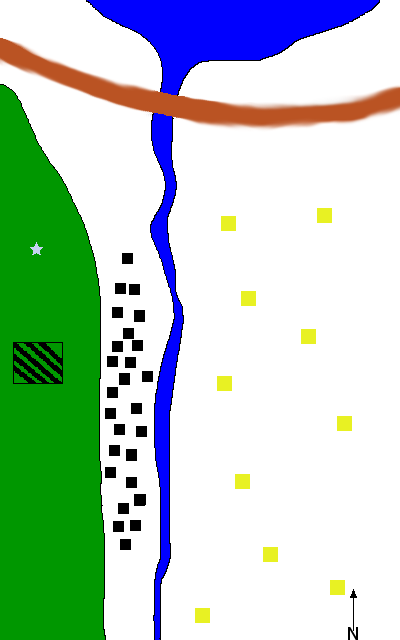
\includegraphics[scale=0.8]{plan.png}
\end{figure}
Il est important de présenter le territoire aux joueurs. C'est un élément important du scénario. 
Il est recommandé de donner une copie de ce plan à vos joueurs (vous pouvez en faire la copie au crayon). 
À l'ouest, il y a le parc naturel national, en son centre, il existe une zone interdite. 
Un esprit très puissant protège cette zone.\\
Au nord-ouest, il y a une mine d'uranium à deux heures de route. Au nord du village, un lac et la grande route. 
L'est est occupé par des grandes fermes et des exploitations agricoles. 
La limite Est du territoire est à 70km du  village: une chaîne de montagne.  
La grande route traverse la chaîne par un col. \\
Au sud du village, le ruisseau prend sa source. Cela monte dans les montagnes. \\

\clearpage

\subsection{Les esprits}
Les esprits sur le territoire sont traumatisés et n'aideront pas les PJs. Ils sont installés depuis un peu plus d'un an et ils n'ont pas de totem (esprits protecteur d'une meute). 
\Jessica n'a pas voulu forcé un esprit à devenir le totem de la meute. Elle attend qu'il y est un candidat. 
Il y a quelques jours, l'esprit gardien de la forêt qui réside dans la zone interdite à envoyer un émissaire à \Jessica. 
L'esprit Gardien demande à la meute de prouver sa valeur en réalisant le rituel de Chasse Sacrée. 
\Jessica a accepté le défi. Le rituel a lieu trois jours après la visite de l'émissaire. Ce défi est le premier geste des esprits locaux pour reconnaître la puissance de la meute.

\subsection{Pour les personnages}
Il est bon de rappeller aux joueurs les quelques informations suivantes en privée.
\begin{itemize}
\item \Lynn : en privée, aborder la questions des absences qui sont assez fréquentes.
\item \Peter : Souhaite devenir maire, il suit des cours de français.
\item \Luke : Rien
\item \Leonard : un sénateur américain et sa famille vont venir, lundi, pour chasser. Cela demande un petit plus en sécurité. Ils souhaitent abattre quelques gros gibiers. 
\item \Jessica : Elle a invité sa meute, ce soir pour le rituel. Le joueur de \Jessica commencera la partie par son RP. 
\end{itemize}

\subsection{Les équipements}
Je n'ai pas l'habitude de dire aux joueurs qu'ils ont de l'équipement, s'il y pense tant mieux sinon il se débrouille sans.
\begin{itemize}
\item \Lynn : Aucun
\item \Peter : Voiture et possibilité d'avoir une arme à feu.
\item \Luke : Pick Up, tracteur, et pleins d'outils dans son garage.
\item \Leonard : Pas d'armes à l'exception un couteau.
\item \Jessica : Moto, klaive et clinique vétérinaire. 
\end{itemize}

\section{La chasse sacrée}
Le scénario commence un samedi soir.
Les Pj effectuent le rite de la \textit{Chasse Sacrée}. Ils chassent un esprit renard/ruse: Tails. \\
L'esprit ressemble à un renard avec les pattes avants bodybuildées. Il a un large sourire, très large un peu à la façon du Chat du Cheshire. La chasse a lieu dans le \textbf{monde des esprits}. Tails part en avance comme le veut le rituel. Il est facile de suivre sa trace \roll{Astuce + calme}.\\
\begin{figure}[!h]
\caption{\label{arbre_mort} Refuge de \textbf{Tails}}
\includegraphics[scale=0.8]{scaring_tree.png}
\end{figure}
En remontant la piste, ils arrivent aux pieds d'un esprit d'arbre mort. Il semble symétrique. Les branches et les racines forment un schéma assez proche.\\ 
L'odeur disparaît dessous les racines. Il est possible de passer sous les racines mais seulement en forme de loup \roll{Se transformerVigueur + survie + instinct primal}. 
Le renard attend dans le creux du tronc, il fera un grand sourire au loup sous lui puis il partira en courant sur une branche et fera un saut géant. 
Faite une course poursuite selon les règles du monde des ténèbres. Le renard à 23 en vitesse, il a une avance de 10 succès, il jette 7 dés pour la course. Il est normalement très difficile pour les joueurs de le rattraper. 
Laissez les espérer.\\ 
Après un ou deux tours de course, le renard saute au dessus d'une crevasse. 
Les loups-garous ne peuvent pas voir ce qu'il y a dans la crevasse, ni sa largeur. Les joueurs peuvent essayer de mesurer la largeur à sauter \roll{Astuce + Athlétisme(saut)} mais en faisant, ils arretent de courrir. 
Le trou fait trois metres de large (Trois succès pour le franchir). 
L'obstacle devrait donner un peu d'avance à Tails. 
Les joueurs vont probablement réfléchir à deux fois avant de sauter la crevasse. Il est possible de trouver en amout ou en aval des points plus étroits.
C'est le monde des esprits, il peut y avoir pleins de trucs... En réalité, il n'y a que l'esprit d'un ruisseau. \\ 

Si un personnage tombe, il est mouillé par l'esprit du ruisseau, c'est tout.\\
Après ce petit contre-temps, ils se remettrent sur la piste du renard, ils ressentent la fin du rituel. Le rituel est cassé, rompu ou inactif. Le rituel n'est pas terminé à cause d'eux, l'explication la plus plausible concerne Tails.

\section{La peur avance}
Ils retrouveront le renard complètement figé (par la peur), il tremble et s'est réfugié sous un rocher. Il est très difficile de lui parler (-7 aux jets sociaux). Il est pétrifié. Les joueurs doivent le comprendre. Un jet en \textbf{astuce + survie} permet de remarquer que l’ensemble des esprits environnant est dans le même état que le renard.\\
Le meilleur comprend également que cela dessine une trajectoire vers le village des joueurs. Cela vient de l'ouest. Les joueurs peuvent suivrent la trajectoire, ils rencontrent un esprit (avançant lentement). 

\section{Monstre Sous le lit}
L'esprit ressemble à un tapis de flammes noires. Il y a deux yeux et une bouche dans ses flammes. Il traite les joueurs d'incompétents: « Si je viens ici, c'est que votre territoire me plaît, vous êtes trop nul pour le comprendre ».
Si les personnages essaient de s'approcher, ils doivent réussir à se contrôler:  \roll{Résolution + Calme}, s'ils échouent alors ils passent en rage mortelle, et fuient. 
Le jet doit être fait tous les 2 mètres et le malus augmente à chaque fois. \\

\begin{tabularx}{100}{|c|X|}
\hline
Distance & malus\\
\hline
20m & Aucun\\
\hline
18m & -1\\
\hline
16m & -2\\
\hline
14m & -3\\
\hline
12m & -4\\
\hline
etc & ...\\
\hline
\end{tabularx} \\

Cela ne représente la capacité passive de l'esprit. Il possède des moyens plus actifs pour provoquer la peur: des bénédictions ou son influence. J'utilise personnellement la discipline Cauchemar de \textbf{Vampire: Le Requiem} pour décrire les effets des pouvoirs de l'esprit (Attention, c'est un esprit aucun lien dans le scénario avec des Vampires ).
Seule, \Lynn n'a pas besoin de faire le jet. L'esprit veut lui parler. 
Il l'entoure de flammes noires, et la remercie (en privé) pour son travail, elle gagne un don «Peur mortelle»  qui pétrifie de peur quelqu'un. La personne est libéré à la désactivation du pouvoir ou s'il subit des dégâts (plus d'information voir section \ref{Peur_mortelle}).\\
A ce moment de la partie, les joueurs auront certainement mis à nue partiellement la nature de l'esprit: la peur. Cependant, ils ne comprendront pas les raisons de sa venue. Ils chercheront à comprendre et enquêteront. 
S'ils enquêtent dans la forêt (mode physique ou spirituel), ils n'apprendront rien. 
S'ils trainent trop, il est souhaitable de leur rappeler leur contrainte temps: Nuit du Samedi au dimanche. Le lendemain, il y a la messe au temple protestant. 
Le rendez-vous incontournable pour la vétérinaire de la ville, du garagiste, du futur maire et actuel Shérif, du garde chasse et d'une institutrice.\\  
S'ils enquêtent dans la ville, ils découvrent les lésions \roll{Astuce + Calme} (chapitre suivant). \\
Quand les joueurs retournent dormir, alors aller au chapitre: La chouette crucifiée (cf. \ref{chouette}). 


\section{Les lésions}
\subsection{Dans le monde physique}
\label{physique_enquete}
Le groupe inspecte donc le village. 
Les lumières de certaines maisons s'allument (il est deux ou trois heures du matin).
Elles restent allumées 5-10 minutes, puis s’éteignent, puis une autre maison pour revenir à la première. 
En réalité, les parents se levent pour réconforter leurs enfants après d'horribles cauchemars. 
Vous pouvez, si vous le souhaitez, décrire la chose de façon à faire croire que le village est 
victime d'un famtôme ou d'une quelconque entité surnaturelle qui allume les lumières.
Si les joueurs décident de parler à une famille, ou à un enfant. 
Le père de la famille les accueillera avec un fusil. Quand les joueurs énonceront le nom de leurs personnages ou que le pere verra les personnes cela ira mieux.
C'est un petit village, tout le monde se connaît.
Le père dira que son fil, sa fille ou les deux ont fait de mauvais rêves. 
Le thème des rêves est très fortement orienté vers les loups (monstres). 
Il n'est pas très cohérent pour des personnes connues de rentrer discrètement dans une maison. Si un enfant voit jour en forme de loup, cela pourrait avoir de graves conséquences dans le contexte actuel.
Ils ne demanderons qu'à aller se coucher et dirons aux PJ: "A demain matin à la messe".
Si vous décidez de laisser rentrer les pj dans une maison, ils se sentiront mal à l'aise. La raisonnance de l'essence dans les maisons est fortement chargée d'émotions négatives (peurs).

\subsection{Dans l'hisile}
\label{hisile_enquete}
Il existe un seul locus sur leur territoire. Ils doivent donc y aller pour outrepasser.
Dans le monde des esprits, le village est enfumé. La fumée vient de presque toutes maisons du village. Cette fumée est grise sombre et elle ne s'élève pas dans le ciel.
Pour s'approcher, les joueurs devront négocier avec l'esprit d'une maison. Il demandera à la meute de réparer les problèmes en échanges du passages (cela peut-être un don d'essence ou une action plus directe sur la famille). \\
L'esprit de la maison demandera à se que les loups-garous soignent la lésion pour les laisser passer (ou de l'essence).\\
Une fois à l'intérieur, la source de la fumée est évidente. Elle vient de l'étage.\\
La fumée descend comme une cascade de l'escalier. Les murs suintent du liquide noir. Le sol est craquelé, comme de la peau brûlée.\\
Il faut essayer de poser une ambiance assez horreur. Les joueurs peuvent remonter la source de la fumée. Cela les guident vers une chambre (d'enfant), bizarrement la chambre n'est pas enfumée. C'est comme l’œil du cyclone. A l'intérieur, il y a 3 esprits : un esprit de sommeil, un esprit de pompier et un esprit d'indien. Ils ont les yeux complement rouge et la peau déformée. Ils attaquent à vue la meute. Le combat est assez facile cependant les joueurs ne seront pas plus avancés. S'ils font plusieurs maisons, ils découvriront la même chose (changé un peu la description des esprits dans chaque maison, mais tous ont muté et sont agressifs). Les détruire n'arrange rien (Caractéristiques des esprits voir \ref{esprit_mutant}). 

\section{La chouette crucifiée}
\label{chouette}
En rentrant chez lui, \Peter découvre qu'une chouette est crucifiée sur la porte de la maison. Elle a été cloué à sa porte vivante et est morte en se vidant de son sang. C'est une espèce protégée. \Jessica ou \Leonard pourront le lui dire. Gérez la chose avec le joueur. Il peut appeler les membres de sa meute ou gérer cela tout seul. S'il enquête, il trouvera des traces de pas et la présence d'un voiture devant chez lui, rien de plus.

\section{La messe}
Le dimanche matin, la ville entière se donne rendez-vous au temple pour la messe et se montrer (Détailler un peu la relation religion/loup-garou). 
Le maire accueille l'ensemble des personnes avec son neveu \Christopher. Il présente son neveu au village. Il vient effectué un stage. Le maire est clairement en campagne électorale, avec 3 mois d'avances. Ils invitent tout le monde à un pique-nique après la messe.
Le serment du pasteur évoque dieu comme un berger, qui protège ses moutons contre les loups. Si vous vous y connaissez, faites-vous plaisir. \\ 
Des trucs clochent, les personnages peuvent remarquer quelques points: \\
Le maire de la ville est très bien habillé (d'habitude, c'est plutôt un bouseux en salopette).\\ 
L'ambiance n'est pas trop à la joie \roll{Astuce + Empathie [caché] }\\  1 succès = Truc louche,\\  2 succès = les gens sont fatigués et stressés,\\  3 succès = les enfants sont absent, cela manque de bruit.\\
Musique: Gospel ou l'hymne du Canada.

\section{Pique-nique après la messe}
Après la messe, le pique-nique commence, le maire fait discours. Les assistants de \Peter glisse un petit mot au maire et à \Peter. Le jeune assistant de \Leonard lui transmet également un fax. C'est un avis de tempête sur la ville. Elle commencera ce soir vers 20h et durera jusqu’à 2h du matin. Le maire prend un mégaphone pour communiquer l'information. Tout le monde part pour aller barricader sa maison. 
Les joueurs doivent faire pareil. La copine de \Leonard, \Elisabeth lui demandera de l'aide. \Luke sera aussi pas mal sollicité. Faite leur gérer cela: \roll{Astuce + Artisanat}.  \\

Vous pouvez placer quelques événements mineurs: Des villageois informent les joueurs qu'il y a des traces de loup un peu au sud du village (vers la montagne). C'est trop tôt dans la saison pour les voir si bas des montagnes.
Puis vient le gros événement, les \Hidden.

\section{Le hurlement des \Hidden}
Le dimanche vers 17h, Les PJ entendent des hurlements qui les appellent.  
Le hurlement dit "Les \Hidden souhaitent rencontrer les \Night ". Vous pouvez signalez à vos joueurs que l'utilisation du nom de votre meute est une vrai marque de politesse et de respect. Aux yeux de beaucoup de loups-garous une meute sans totem n'est pas une vrai meute. 
L'appel vient de l'est et de loin (à environ 70km, la frontière de leur territoire). Il est préférable d'y aller en véhicule par la grande route.

\section{La rencontre avec \Hidden}
Le lieu de rencontre est un petit col, à la frontière Est du territoire. 
Il est possible d'y accéder par la grande route.
Les PJ rencontrent la meute des \Hidden. Laissez choisir comment ils abordent la rencontre: 
Garer la voiture à proximité, faire une réconnaissance par l'irraka d'abord, etc.\\ 
Les \Hidden sont quatre, trois hommes et une femme.
Ils expliquent qu'un membre de leur meute est devenu fou. 
Il a tué de nombreux humains, et a violé beaucoup de points du serment de la Lune. 
Il est devenu un \Thomas. Un loup garou ayant une harmonie très basse voire nulle. \\
Les \Hidden pensent que ce danger est sur le territoire des joueurs. Ils préfèrent prévenir. 
Les \Hidden resteront polis, afin d'attirer le moins possible l'attention des joueurs. \\
Un des membres de la meute est blessé, il lui manque deux doigts (annulaire et auriculaire de la main gauche). 
Il se justifie en disant que le \Thomas est responsable de sa blessure. Il lui a mangé les doigts. 
Les \Hidden donneront une photo en forme humaine du \Thomas.\\
Si les joueurs invitent les \Hidden, ils refuseront poliment. 
Si les joueurs insistent, ils accepteront mais partiront dès que possible.
Quand les joueurs retournent au village, la tempête commence, de fortes pluies. 
Vous pouvez tester leur conduite \roll{Dextérité + Conduite} avec un malus pour le mauvais temps. 
J'utilise aucun malus, s'ils ont pris une voiture. Si \Jessica a pris sa moto, j'applique un malus de -2 dés.\\
Bref, les joueurs rentrent au village. la tempête gagne en puissance. 
Le village est comme mort. A ce moment là, normalement vous avez croqué le cerveau de vos joueurs.  
Musique: Tension


\section{Pendant la tempête}
Vous pouvez ici jouer quelques scènes d'actions, facultative.\\
Soit:\\ 
\begin{itemize}
\item  \Elisabeth joue à des jeux sado-maso avec \Leonard (elle pourrait voir sa régénération surnaturelle, attention à la lubie).
\item \Elisabeth est possédé par l'esprit de peur (\Monster) et elle obtient une voie qui pétrifie \Leonard. Il ne revient pas vers les autres à la fin de la tempête. Les autres joueurs s'inquiéteront de son absence.
\item \Peter apprend qu'un enfant a fuit sa maison pendant la tempête. La meute ira certainement le sauver.
\item Un incendie se déclare à la fin de la tempête, il brûle une maison et menace de se répandre à la seule pompe à essence de la ville. 
\end{itemize}
Quoi que les personnages font, ils peuvent entendre \roll{Astuce + Calme} une meute de loups assez importante hurler. Les hurlements s'arrêteront assez brutalement. La tempête continuera quelques heures après les hurlements. \\
Si les personnages sortent pour enquêter dans la tempête, faites les souffrir. C'est une très mauvaise idée de sortir pendant une tempête. S'ils y vont pour sauver un enfant, vous pouvez être plus sympa. L'enfant ne se sera pas enfoncé trop loin dans le parc naturel.\\
C'est à vous de meubler ce passage ou de le faire vite passer.

\section{Une meute de loup est retrouvée morte}
\label{MeuteMorte}
Les personnages voudront probablement enquêter sur cette meute, après la tempête. C'est peut-être elle qui vient proche du village et fait peur à des enfants? (ce n'est pas sur que les joueurs aient compris cela) \\
Il est difficile de s'orienter dans la foret après la tempête \roll{Astuce + Survie}. Au termes de leur traque, ils trouveront des cadavres de plusieurs loups dans la forêt du parc naturel. \\
Enquêter leur permet de comprendre les choses suivantes \roll{Astuce + Survie ou investigation} : \\
-Une louve de la meute est encore en vie.\\
-Dans un recoin, un loup blessé s'était réfugié (une odeur de sang mais la tempête a effacé toutes les traces).\\ 
-La meute l'a encerclé pour attendre sa mort avant de le manger.\\
-Les loups ont perdu patience et il y a eu un combat. Le loup(-garou) a pris une forme plus forte (gauru). 
il est passé à l'attaque. Il a détruit la meute de loup. Certains loups de la meute se sont enfuit. \\
La rage mortelle de l'individu peut troubler les esprits environnant. Ils ne seront pas coopératif et critiqueront l'efficacité des joueurs. Si un don quelconque est utilisé pour revoir la scène, l'image devient noire. L'esprit a eut peur, il a "fermé les yeux".\\
L'utilisation de langue animale et témoignage de cadavre permet d'avoir la fuite du \Thomas.\\
-Il y a un schéma qui se dessine dans la foret. Le loup-garou ne semble pas avoir tué volontairement les loups. Beaucoup sont morts écrasés sous le poids du gouru. Après s’être transformé, il a pris la fuite vers l'ouest (extérieur de territoire des joueurs). \\
1 - Il a perdu sa forme gouru après 50 mètres.\\
2 - Il se cogne contre quelques arbres et avance difficilement en zigzagant.\\
3 - Il se transforme en gouru. Il plie des arbres sur son passage en gouru. (on repart sur l'étape 1).\\
Ce schéma est répété plusieurs fois, puis la trace remonte dans la montagne, il y a plus d'arbre et que des rochers, la pluie a tout effacé. De plus, la trace se perd à quelques centaines de mètres de la fin de leur territoire.\\

A ce moment, il y a deux possibilités. Soit vos joueurs voudront continuer sur la piste même si elle est perdue (la direction générale mène vers la frontière du territoire). Soit ils voudront sauver la louve.\\
Dans le premier cas, vous pouvez aller directement consulter le chapitre: \ref{sadness}, sinon aller voir \ref{louve}.
Musique : Foret 



\section{La louve}
\label{louve}
Un jet de \textbf{dextérité + médecine} pour soigner la louve est possible. 
La louve a perdu une patte, ce détail est important. \\ 
Cette étape est juste, un moyen de décompresser un peu et de regrouper la meute, si elle ne l'était pas. 
C'est très probablement la vétérinaire qui voudra soigner la louve. 
Une meute part rarement en chasse sans son alpha. 
Le temps de gérer la louve. C'est le lundi matin. 
Il faut gérer les conséquences de la tempête [chapitre: \ref{consequence} ]. \\


\section{Tempête: les conséquences}
\label{consequence}
Cette section est un peu un moment bac à sable. Si vos joueurs ont raté des indices, c'est le moment de la séance de rattrapage. \\
-Vous pouvez jouer le chapitre \ref{hisile_enquete}. S'ils n'ont pas visité de lésions avant.\\
-Pareil pour \ref{physique_enquete}, les gens se montrerons sûrement plus bavards. Il est possible d'apprendre que certains enfants parlent d'un loup à leur fenêtre. Une enquête \roll{Astuce + investigation} montrera qu'un loup-garou en Urshul s'est agrippé au rebord de la fenêtre. Il regardait dans la chambre.\\
-Certaines familles vivants dans le sud (dans les montagnes) parleront de loup à 3 pattes qui pillent les poubelles.\\
-Les plus gros dégâts sont enregistrés chez la famille: Porkman. Ils ont des triplés. Les enfants jouaient dans la grange, quand elle s'est effondrait, 
ils ont eut le temps de partir dans la maison (en bois), qui s'est effondré à son tour. Ils se sont réfugiés dans la dépendance en brique de la maison.\\
Il ne faut pas hésiter à demander aux joueurs d'avoir des idées pour calmer les peurs des enfants. La tempête a ravagé la ville. Les lésions sont encore plus grandes. Atelier peinture, réunion d'informations, tout est possible mais rien ne marchera vraiment mais c'est mieux que rien.

\section{Le sénateur du Texas chasse}
Le lundi à midi, le gouverneur arrive avec sa fille et son futur gendre. Ils vont chasser en forêt. \Leonard doit les accompagner vers un point de vue où ils s'installeront pour chasser. Le père et la fille savent chasser et ont l'habitude des armes. Le gendre est beaucoup moins à l'aise. 
La forêt est en bordel, \Leonard doit réussir un jet de \roll{Astuce + Survie} pour trouver une route vers la zone. \\
Le sénateur va voir une chose au loin et va tirer. \\
Sur le chemin, le gendre identifie des traces bizarres. C'est gris. On en voit sur des trons et par terre. Le gouverneur (un homme rond et vieux) pense que c'est des excréments d'animaux mais ne connaît pas le type. Si \Leonard (ou un autre loup garou) touche cette substance, cela chauffe dans ses mains. S'il le renifle, il se prends un dégât aggravé et un mal de tête monstrueux. Il ne faut pas oublier de faire un jet de rage mortelle. La transformation en gouru annule les malus de douleur et détruit l'argent de l'organisme.\\
\Leonard porte le gros du matériel. Ils laissent les 3 chasseurs dans un point de vue et repart.\\
Cette scène est un moyen de raccrocher les joueurs sur la piste du Monstre (le Zi'ir). Si vous voulez la rendre plus intense, vous pouvez. Vous pouvez soumettre l'idée que \Leonard demande à la meute de se réunir vers la piste pendant que lui, finit avec les chasseurs. 


\section{Sur les traces du \Thomas}
Le beau temps et les blessures du \Thomas le trahissent. Il est maintenant possible de le suivre et de comprendre un peu son comportement. En fait, il vient dans la forêt pour se nourrir mais ne vit pas sur le territoire de la meute mais juste à la frontière. La trace identifié par Léonard mène droit vers la grotte. Les joueurs seront très enthousiaste à l'idée de l'attaquer.
Ils vont vite déchanter (voir \ref{black_eclipse} ). 
Quand vos joueurs auront retrouver les traces qui mènent vers le \Thomas, laisser leur le temps de se regrouper pour élaborer une stratégie. Le \Thomas est dangereux dans leur tête (c'est le boss de fin pour eux). 



\section{\BlackEclipse attaque}
\label{black_eclipse}
Les personnages courent en suivant la piste du \Thomas. Elle mène vers l'Ouest du territoire. Quand ils ne sont qu'à quelques kilomètres de la fin de leur territoire, faite leur faire \textbf{un jet d'Astuce + Calme - malus d'environnement} (Si un personnage est en avant par rapport aux autres, C'est lui qui fait le jet et subit l'attaque). Ce jet permet de savoir s'il est surpris (pas de défense) ou non. Heureusement pour eux, il n'y a qu'un attaquant. \\
\BlackEclipse aura le temps de faire une seule attaque (Elle a l'initiative obligatoirement, au premier tour). Elle est en forme gauru et elle attaque avec ses griffes, elle n'a que 12 dés d'attaques. Elle ne tuera pas volontairement, son but est de les interdire de remonter la piste. Elle veut protéger son fils (le Zi'ir).\\
Quand elle a attaqué, elle est assailli par deux loups-garous en forme \textit{Urshul} (\textbf{Vicious Pain et Red fangs} (voir \ref{sadnessknives})), les deux autres se positionnent en Dalu entre le trio et la meute des joueurs. \textbf{Fair Wolf} utilisera \textbf{Aura de trève} pour calmer tout le monde.
\BlackEclipse va se calmer et se changer en Dalu. C'est une femme d'environ 40 ans, très musclée. Elle a vraiment une tête de vétéran. Dans son dos, une hache immense, un fétiche très très puissant (voir \ref{devoreuse} ). Elle ne parle pas avec la meute des joueurs et s'éloigne un peu. Elle passe ses nerfs sur un arbre. Elle gronde vers \textbf{Fair Wolf} en disant "qu'ils n'ont pas à intervenir dans cette histoire". \\ 
\textbf{Fair Wolf} se présente comme le porte parole de la meute des \textbf{Sadness Knives}. Il demande à tous de prendre une \textbf{"forme plus propice au dialogue"}. Quand les joueurs sont en forme humaine ou dalu, faite faire un jet en \textbf{Astuce + Empathie} à tout le monde sauf \textbf{Cendre Griffe}, un succès indique qu'il y a un air de ressemblance entre \textbf{Fair Wolf} et \textbf{Cendre Griffe} (Attention, le joueur de Cendre Griffe, ne doit pas savoir le résultat du test). \textbf{Fair Wolf} va prendre quelques secondes en regarde \textbf{Cendre Griffe} pour lui dire :  {\Large \textbf{Luke, je suis ton père}} avec une petite musique dramatique en fond. \\
Passé cette référence, \textbf{Fair Wolf} demande pardon pour avoir franchi le territoire des joueurs et il lâche des infos. \\
Il explique qu'il y a 10 ans environ, ce territoire était celui de sa meute.\\
Un jour, ils sont partis à la chasse à l'extrémité du territoire, à leur retour, l'enfant de \BlackEclipse avait disparu. Elle est devenue folle et a détruit définitivement le totem de la meute, un esprit Ours/force avec sa hâche. \\
Le totem avait pour mission de protéger l'enfant. Cela a traumatisé les esprits de la zone. Ils ont abandonné le territoire et sont allés s'installer dans Ouest (a des milliers de kilomètres). Il y a quelques jours, \BlackEclipse a eut des visions et elle est retombée dans sa folie à propos de son fils. Ces visions lui montraient son fils adulte dans le village des Joueurs. Elle a donc quitté le territoire pour se rendre ici. Il est important d'expliquer qu'elle est dans la zone depuis plusieurs jours. Elle a été rattrapé par sa meute, qui lui a fait entendre raison. Elle repartait quand elle a entendu le coup de feu (tiré par le sénateur). 
Elle a voulu aller voir et a trouvé les \Night. \\
C'est une petite astuce pour expliquer pourquoi, elle apparaît maintenant et pas avant.\\

\section{Black Eclipse Vers son fils}
Laissez vos joueurs réfléchir avec les nouvelles données qu'ils viennent d'obtenir. 
Si cela traîne trop, les \Sadness demanderont au joueurs de les accompagner à la frontière pour leur montrer qu'ils ne sont pas des ennemis. Les deux meutes suivent donc la piste, \BlackEclipse pense que c'est son fils, mais rien n'est sur.\\ 
Si les joueurs parlent, des \Hidden et montre la photo. \BlackEclipse prendra la photo et tombera en larmes. \\
A la frontière du territoire,  les deux meutes se séparent.\\
Il est temps de recentrer l'action sur l'esprit de peur. Il y a plusieurs possibilités soit vous relancez un peu l'enquête sur l'esprit de peur soit vous déclenchez le chapitre suivant. \\
Personnellement, je profite de ce temps pour faire un point avec les joueurs de ce qu'ils savent et des interrogations qu'ils ont. \\


Après que les joueurs aient réfléchi à un plan d'actions et qu'ils redescendent vers le village. Lancez la suite!


\section{Fin possible}
Cette section a pour but de vous donner un peu de recul face à l'histoire. A ce moment de la partie, vous joueurs auront compris (à tord) que \Thomas fait peur aux enfants du village. Il n'est pas la seule cause des peurs et c'est à vous de le faire comprendre aux joueurs, ou du moins d'essayer. Ne les laissez jamais rester trop enquêter sur la même piste. Ils vaut mieux les mélanger un peu. La fin que je propose est une fin possible qui me semble raisonnable. Sentez vous libre de la modifier. Je fais le choix délibérer de ne pas faire un grand combat épique à 3 meutes (ou 2) cela serait bien trop long. Je laisse un adversaire dangereux, voir: \ref{ausecours}.
Vous pouvez faire le choix de laisser 2 adversaires au lieu d'un. J'aime que \textbf{Winter Mist} s'échappe cela sert de Cliffhanger au scénario. Partez du principe que l'action des joueurs peut changer la donne. C'est difficile mais rien n'est impossible.

\section{Night Howler au secours!!}
\label{ausecours}
Cette scène est à placer au bon moment dans la partie. Elle peut intervenir le lundi matin juste  après la scène \ref{black_eclipse} ou bien après. 
Ils apprennent que des quelques choses ne va pas. Cela peut être \Tails l'esprit de la foret qui les prévient que des loups-garous sont passés par leur locus. Cela peut être des coups de feu tiré par le sénateur alors que les joueurs sont dans la forêt. Cela peut être un hurlement de demande à l'aide. \\
Des loups-garous ont utilisé leur locus pour passer de l'hisile au monde réel et ont pris direction plein Ouest. Ils sont 4. Que les joueurs remonte la piste ou courent pour aller aider les personnes qui les appellent à l'aide. \\
Ils vont aller au delà de leur territoire. En redescendant la chaîne de montagne, ils vont voir de loin une scène d'horreur. 
\textbf{Winter Mist} est derrière \BlackEclipse. Elle est à genoux et sévèrement blessée. Les personnages courent dans la direction de la zone mais ils sont encore trop loin. Ils voient \textbf{Winter Mist} décapiter la pauvre femme et mordre dans la joue de la tête découpée. Il a visiblement orchestré la scène pour que les joueurs voient ça. Il parle à un membre de sa meute (Unwise Wolf) qui se met en position et attend les personnages toutes mâchoires et griffes en argent dehors. \textbf{Winter Mist} et un autre membre de sa meute utilisent la vitesse de père loup pour s'enfuir. Il faut gérer le combat et/ou la course poursuite.  

\section{La scène de crime}
Une fois le combat terminé, les joueurs vont probablement avoir envie de comprendre ce qui s'est réellement passer. Il y a un membre des \Hidden mort par terre. Quatre membres des \Sadness sont morts. Il manque donc une personne \textbf{Vicious Pain}. 
Laissez les gérer la scène de crime \roll{Astuce + investigation (scène de crime) }. Il est possible de comprendre que les \Hidden sont tombés par surprise sur les \Sadness. Ils ont utilisé des armes en argent visiblement. Ils étaient clairement bien préparer. La hache est brisée et l'esprit a été libéré. \textbf{Vicious Pain} n'est pas là. Son corps est un peu plus loin devant une grotte (\ref{chirurgie}). potentiellement dire qu'il est toujours bon d`enterrer des Uratha et leur rendre un dernier hommage. S'ils n'ont pas réalisé qu'il manque une personne ou s'ils ont fait pas mal de succès pour enquêter. 

\subsection{Alternative: La hache n'est pas brisée}
Il peut être intéressant de jouer un combat entre les \Hidden et les joueurs pour savoir qui gardera la hache. Les \hidden ne seront pas en état de tenir le combat très longtemps et fuiront. Le gage de sagesse serait de libérer l'esprit à l'intérieur et de détruire l'arme. Cette arme traumatise les esprits environnants.

\section{Chirurgie au Klaive}
\label{chirurgie}
Le \Thomas est dans une grotte, il est difficile d'y voir un truc sans s`approcher. Il a un comportement assez étrange. Il change de forme assez continuellement: de forme humaine, urshul, dalu et Gauru. Une énorme bosse est visible dans son dos. Il se jette contre la paroie de la grotte, la bosse en avant. Il est évident que cela provoque de la douleur.   Un jet en \textbf{Astuce + Occultisme} permet d'identifier les marques d'un rituel dans les tatouages entourant la bosse.
Normalement, ces informations devrait suffire aux joueurs pour comprendre qu'ils peuvent sauver le \Thomas. Il faut l`immobiliser, ouvrir la "bosse" et en retirer le catalyseur de douleur. C'est à \Jessica de faire le travail probablement.
Ce n'est pas compliquer. Ils peuvent prendre quelques dégâts dans l'opération mais rien de méchant. Il faut les faire stresser un peu quand même. \\
Une fois, le sujet immobilisé, faire un jet en \textbf{Dextérité + Arme blanche (rituel)} pour découper la bosse et ouvrir la zone. La bosse est pleine de pus et il y a au milieu, deux pièces brillantes (des griffes en faite), il faut les arracher. Dès qu'elles ne sont plus dans le corps, elles prennent une forme de doigt.

\section{Les enfants}
Le lundi matin ou le mardi matin.
A ce stade, les joueurs auront compris que c'est la peur des enfants qui nourrit l'esprit.
Dans le monde des esprits, l'esprit est beaucoup plus gros, il se multiplie formant comme un réseau pour absorber l'ensemble de l'essence. Il entretient la peur. En général, les joueurs commencent à fatiguer et veulent du réel. Il est important de finir une ou deux intrigues. Laissez les joueurs avoir de l' imagination, pour faire parler les enfants. Il est possible d'apprendre que certains enfants rêvent de la même chose. 
Un loup a 3 pattes, un loup à leur fenêtre, des loups dans la forêt s'approchant des maisons. Il est possible qu'un des rares élèves présent le lundi ou le mardi signale le tableau bizarre dans la classe de \Lynn . 

\section{Le tableau dans la classe}
Pendant l'absence de \Lynn le vendredi soir. Un esprit lui a fait placer un de ses tableaux dans sa salle de classe. \Lynn est incapable de le voir, cela ne la choque pas. Les enfants ne le verront qu'à partir de Lundi. Tous les enfants présents le lundi ne seront pas là le jour suivant. 
Il est possible que le joueur de \Lynn décide de parler des ses moments d'absence aux autres. 
Si \Jessica apprend pour le tableau, vous pouvez lui faire faire un \textbf{jet de rage mortelle} contre \Lynn . Si les joueurs parlent avec des élèves de \lynn, ils auront grandement peur d'elle.
Si le joueur de \Lynn ne parle pas, consultez la section \ref{directeur}.

\section{Directeur de l'école}
\label{directeur}
Cette scène peut-être joué à partir du mardi matin. C'est une section bonus pour donner des indices. Il est très rare que la démarche des joueurs auprès des enfants leur permette d'apprendre cela avant. 
Le directeur aura reçu beaucoup de courriers ou de coups de fil. Des parents d'élèves se sont plaint du nouveau tableau de la salle de classe. Visiblement, il provoque des cauchemars chez les enfants. Le directeur confirmera; le tableau n'a rien à faire dans son école et demandera donc des explications à \Lynn. Il est possible pendant l'interview avec le directeur de voir que \Elisabeth est aussi concernée par les demandes des parents d’élèves.


\section{le cas \Elisabeth}
Son emploi du temps avec les enfants est simple. Elle leur lit des contes en français tous les après midi. Elle est influencée par \Monster . Il lui donne un pouvoir de manipulation des rêves. Sa voix influence grandement les rêves de son auditoire. Elle lit des contes assez sanglants et tristes. Les élèves ne comprennent pas tout mais le pouvoir n'a pas besoin de ça. \\ 
Elle est très attaché à un livre. \\ 
\Monster fait en sorte qu'\Elisabeth aime particulièrement ce livre de conte (une copie d'un ouvrage du 14ème siècle). Il est en français donc il faut faire un jet en \textbf{Intelligence + Érudition}. Seul \Peter et \Lynn ont des notions de français. \\

Du coup, si \Elisabeth parle à \Leonard de jeu sexuel qu'elle voudrait expérimenter, il rêvera de cela. \\

Il y a plusieurs moyens de gérer son cas. Les PJ peuvent décider de la tuer. Il peuvent juste l'enfermer loin des enfants que son influence diminue. \\ 

\section{Les Loups dans la ville}
Des meutes de loups semble de plus en plus s'approcher des habitations. 
Un père de famille a été tué par une meute alors qu'il était sortie pour une raison quelconque. 
La meute est rentré, à tuer toute la famille ou presque. Un enfant a survécu. Il témoignera qu'un Grand loup a combattu les autres et les a repoussé.\\
Cette scène n'a jamais été joué mais je pense que c'est une bonne idée. Pour des raisons de cohérence, j'imagine assez bien la même meute que pour la scène \ref{MeuteMorte} . Ce 
n'est pas obligatoire mais il faut laisser des indices pour inculper ou disculper la louve: Présence d'un loup à 3 pattes. \\ 
Je pense que la scène doit avoir lieu avant la scène \ref{MeuteMorte} mais les PJ pourrait l'apprendre après.  \\
C'est évidemment \BlackEclipse qui aura sauver le petit enfant de 8 ans de la maison. La meute aura fuit devant la présence du loup-garou. L'enfant sera terrorisé, il ne pourra pas dire grand chose mais des cadavres de la maison se montreront peut-être plus bavards. 
Les loups sont agressifs car ils ont peur, cette peur naît de la présence de l'esprit. Ils n'y sont pas vraiment pour grand chose. 
Il n'est pas à exclure que \BlackEclipse se soit battu contre les loups sans les blesser, uniquement pour les repousser violemment afin de sauver l'enfant. Pendant le combat, elle a pu être blessé. C'est à ce moment que sa meute est arrivé pour l'arraisonner. 



\section{Le maire de la ville}
\label{le_maire}
Il est possédé par un esprit de Chicago. Il cherche à faire payer à \Peter le prix de ses actions. En effet, la mort des vampires a entraîné une guerre de succession et une guerre de gang. Ce n'est pas bon pour le business. Son neveu était le vecteur de l'esprit.
L'esprit a possédé \Christopher de Chicago jusqu'au village, puis il a pensé que le maire était une meilleure cible pour une possession. \\
\subsection{Les indices du monde des esprits}
Durant leur investigation dans le monde des esprits les joueurs pourraient voir des choses étranges autour de la maison du maire. \\
Elle se transforme petit à petit en building de grande ville. Des fumées sont visibles autour de la maison. Des klaxons sont audibles, des taxis jaunes circulent dans la fumée. 
L'entrée de la maison ressemble au hall d'entrée d'un building. Il y a un vrai labyrinthe d’ascenseur pour arriver dans les parties vivables de la maison, les chambres, et la chambre de \Christopher. Il peut être marrant d'utiliser un taxi pour prendre l'ascenseur les couloirs etc. Il faudra bien sûr payer la course. \\
Il est possible d'interroger l'esprit de la maison pour obtenir les informations (voir \ref{Julian}). Il est possible que les enfants du maire soient victimes des peurs. 

\section{Les récompenses}
Quand  tous les problèmes auront été réglé: les peurs, \Monster, le maire, \Elisabeth et  la tempête. 
L'esprit protecteur de la forêt apparaîtra devant la meute pour les remercier. \\
L'esprit gardien est un dragon de bois, sa peau est faite d’écorce d'arbre. 
Ses ailes sont faite de branches. Son dos baigne dans la lumière et toutes sortes de mammifères y vives: 
Cerfs, écureuils, Sanglier, renard, souris. Son ventre représente la nuit, des insectes y grouillent; 
il y a des milles-pattes, des araignées et toutes sortes d'insectes.
Il est le gardien de la \textbf{Clairière} qui se trouve être dans le parc. 
Il reconnaîtra la sagesse, l'honneur et la pureté de la meute.
Il a vu les qualités de la meute. La meute aura plus de facilité à obtenir un totem.
Tails fera un grand sourire aux pieds de l'esprit gardien à ce moment.\\

\chapter{La vérité}

\section{Raison de la présence du \Monster}
Il y a principalement trois raisons de sa présence et des secondaires: 
\begin{itemize}
\item \BlackEclipse : Inspecte les maisons pour y chercher son fils, souvent en forme de loup. Les enfants la voient, et ils ont peur.
\item \Elisabeth : Elle Raconte des contes horribles aux enfants, elle est influencée par l'esprit \Monster.
\item Le tableau dans la salle de cours de \Lynn. 
\item Une grande meute de Loup se rapproche du village pour manger.
\item La tempête
\item ce que vous voulez...
\end{itemize}

Les fausses pistes:
\begin{itemize}
\item \Thomas est dans la zone, il souffre d'un rituel. Deux ongles en argent sont sous sa peau. 
Cela le rend fou de douleur. Il n'est pas du tout un Zi'ir. Il est incapable de se contrôler mais il a réussi à 
s'isoler. 
\item Le maire est possédé par un esprit de la ville de Chicago. Il veut se venger de \Peter. C'est un problème qu'il faut gérer, mais il n'y a aucun rapport avec les peurs.
\end{itemize}


\subsection{\Lynn et son aide}
Vendredi soir, \Lynn a été possédé par un esprit de Lune corrompu. 
Cet esprit n'est pas l'objet de ce scénario mais vous pouvez ajouter cette intrigue si vous le voulez. 
Le Sélène est un cahalumine qui a fait une alliance avec \Monster .


\chapter{Annexes}
\section{PNJ Importants}
\subsection{Les esprits mutants}
\label{esprit_mutant}
\paragraph{L'esprit du Sommeil}
\begin{itemize}
\item Puissance : 2
\item Finesse : 7
\item Résistance : 5
\item Volonté : 7
\item Taille : 4
\item Corpus : 9
\item Essence : 15
\item Défense : 7
\item Initiative : 12
\item Vitesse : 4
\item Influences : Sommeil 2
\item bénédictions: Vision matérielle, télékinésie (P.66 predators),Entrave, Portée, Éclair (il envoie des plumes orange comme le pus). 
\end{itemize}

\paragraph{L'indien}
\begin{itemize}
\item Puissance : 2
\item Finesse : 4
\item Résistance : 2
\item Volonté : 6
\item Taille : 3
\item Corpus : 5
\item Essence : 10
\item Défense : 4
\item Initiative : 6
\item Vitesse : 10
\item Influences : Indien 1
\item bénédictions: Déluge, décorporation, vision matérielle.
\end{itemize}


\paragraph{Le pompier}
\begin{itemize}
\item Puissance : 5
\item Finesse : 2
\item Résistance : 4
\item Volonté : 9
\item Taille : 6
\item Corpus : 10
\item Essence : 13
\item Défense : 5
\item Initiative : 9
\item Vitesse : 8
\item Influences : feu 1, jouet 1
\item bénédictions: diriger le feu, vision matérielle, Entrave, Portée.
\end{itemize}

\subsection{Les assistants}
\begin{tabularx}{\linewidth}{|c|c|X|}
\hline
Nom & Rôle & Description \\
\hline
Collin & Assistant de \Peter & Homme, 40 ans, grand et solide, un peu lent à la détente. Il est timide mais ne se laisse pas marcher sur les pieds\\
\hline
Dustin & Assistant de \Peter & Homme, 30 ans, Mince et vif. C'est un frimeur et un beau parleur.\\
\hline
Grant & Assistant de \Leonard & Jeune homme de 17 ans, un peu hippy sur les bords.  \\
\hline
\end{tabularx}

\clearpage

\section{FAQ \& incohérence}
Cette section clarifie des détails. Le but est de favorisé l'improvisation, si vos joueurs sont forces de propositions.
\subsection{Pourquoi il n'y a pas de sang ou de poudre d'argent quand on trouve la meute de loup?}
-A cause de la tempête, elle a tout effacé. 
\subsection{Quels événements sont indépendants de l'action des joueurs et quelle est la chronologie?}
-Le scénario commence le samedi soir, le dimanche matin, il y a la messe, le dimanche soir la tempête, 
lundi les conséquences de la tempête et le lundi midi le sénateur texan. Le lundi comme le mardi, 
il y a peu d'enfants en classe. 
\subsection{La chronologie de la disparition de Thomas.} 
-Thomas a été enlevé à l'âge de huit ans. Il est resté dix ans sans sa mère. 
La meute des \Hidden lui a fait un véritable lavage de cerveau. Deux semaines avant le début du scénario, 
il a été lâché proche du territoire. Il est dressé à tuer à vue les \textbf{Sadness Knives.}
\subsection{Prise de liberté avec les règles.} 
-Il est vrai que je joue beaucoup avec les règles. Les personnages sont plus taillés pour correspondre à 
leur histoire, qu'aux règles de création de personnage.
\Jessica  n'est probablement pas assez expérimentée pour maîtriser le rituel de la \textbf{Chasse Sacrée},
le joueur n'est pas au courant qu'il maîtrise des rituels.
C'est mieux ainsi, les rituels sont important dans le jeu mais trop compliqué à mettre en place pour un oneshot.
Si vous jouez ce scénario intégré dans une campagne, n'oublie pas de prendre en considération cet aspect.

\clearpage

\section{Les règles homemade et création}
\subsection{Don: Peur Noire}
\label{Peur_mortelle}
\don{Peur Noire}{Immobilise un adversaire. L'effet s'estompe quand une des conditions suivantes arrive:
\begin{itemize}
\item A la fin de la scène
\item La victime reçoit un dégât. 
\item l'utilisateur désactive le don. 
\end{itemize}}{Présence + Intimidation + Gloire}{1 point d'essence}{Aucune}{Réflexe}


\subsection{Rituel: Douleur d'argent}
Le rituel de \textbf{Douleur d'argent} est l'ultime façon de faire souffrir un Uratha. 
Il consiste à faire ressentir en continue la malédiction de Mère Lune.
Le sujet reçoit en permanence une faible quantité d'argent dans son métabolisme. 
La douleur pousse le sujet à rentré en Kuruth. La forme gouru associée à la rage mortelle brûle l'argent dans le corps.
La victime du rituel peut alors reprendre une autre forme. La douleur reprend ses droits et cela boucle. 
L'individu préfére bien souvent se suicider plutôt que de continuer à souffrir.

\subsubsection{Réaliser le rituel:}
Le sujet s'allonge sur le ventre. Le ritualiste chante les raisons de ce rituel. 
Le reste de la meute est autour du sujet, le maintenant. 
Un membre de la meute doit utiliser le don \textbf{Mâchoire d'argent}. Il transforme ainsi sa marchoire et ses griffes en argent.
Le ritualiste réalise une incision sur le sujet. 
Il sectionne alors deux droigts de l'utilisateur de \textbf{Mâchoire d'argent} et les place dans la plaie dorsale du sujet.
Toutes les personnes présentent pendant le rituel font un jet de dégénérescence pouvant résulter à la perte
d'un point d'harmonie.

\subsection{Fétiche: Lame Dévoreuse}
\label{devoreuse}
La Lame Dévoreuse est une  grande hache de guerre. 
Un esprit de Sangsue/gourmandise est emprisonné à l'intérieur. 
L'arme ne nécessite aucune activation. Elle donne un bonus de 4 dés pour l'attaque (comme une hache normale).
Les 10 et les 9 se relancent. 
Tout succès provoque un dégât létal et le vol d'un point d'essence. Si la cible n'a pas d'essence (ou équivalent),
cela inflige un dégât supplémentaire.  




\section{Carte heuristique}  
\begin{figure}[!ht]
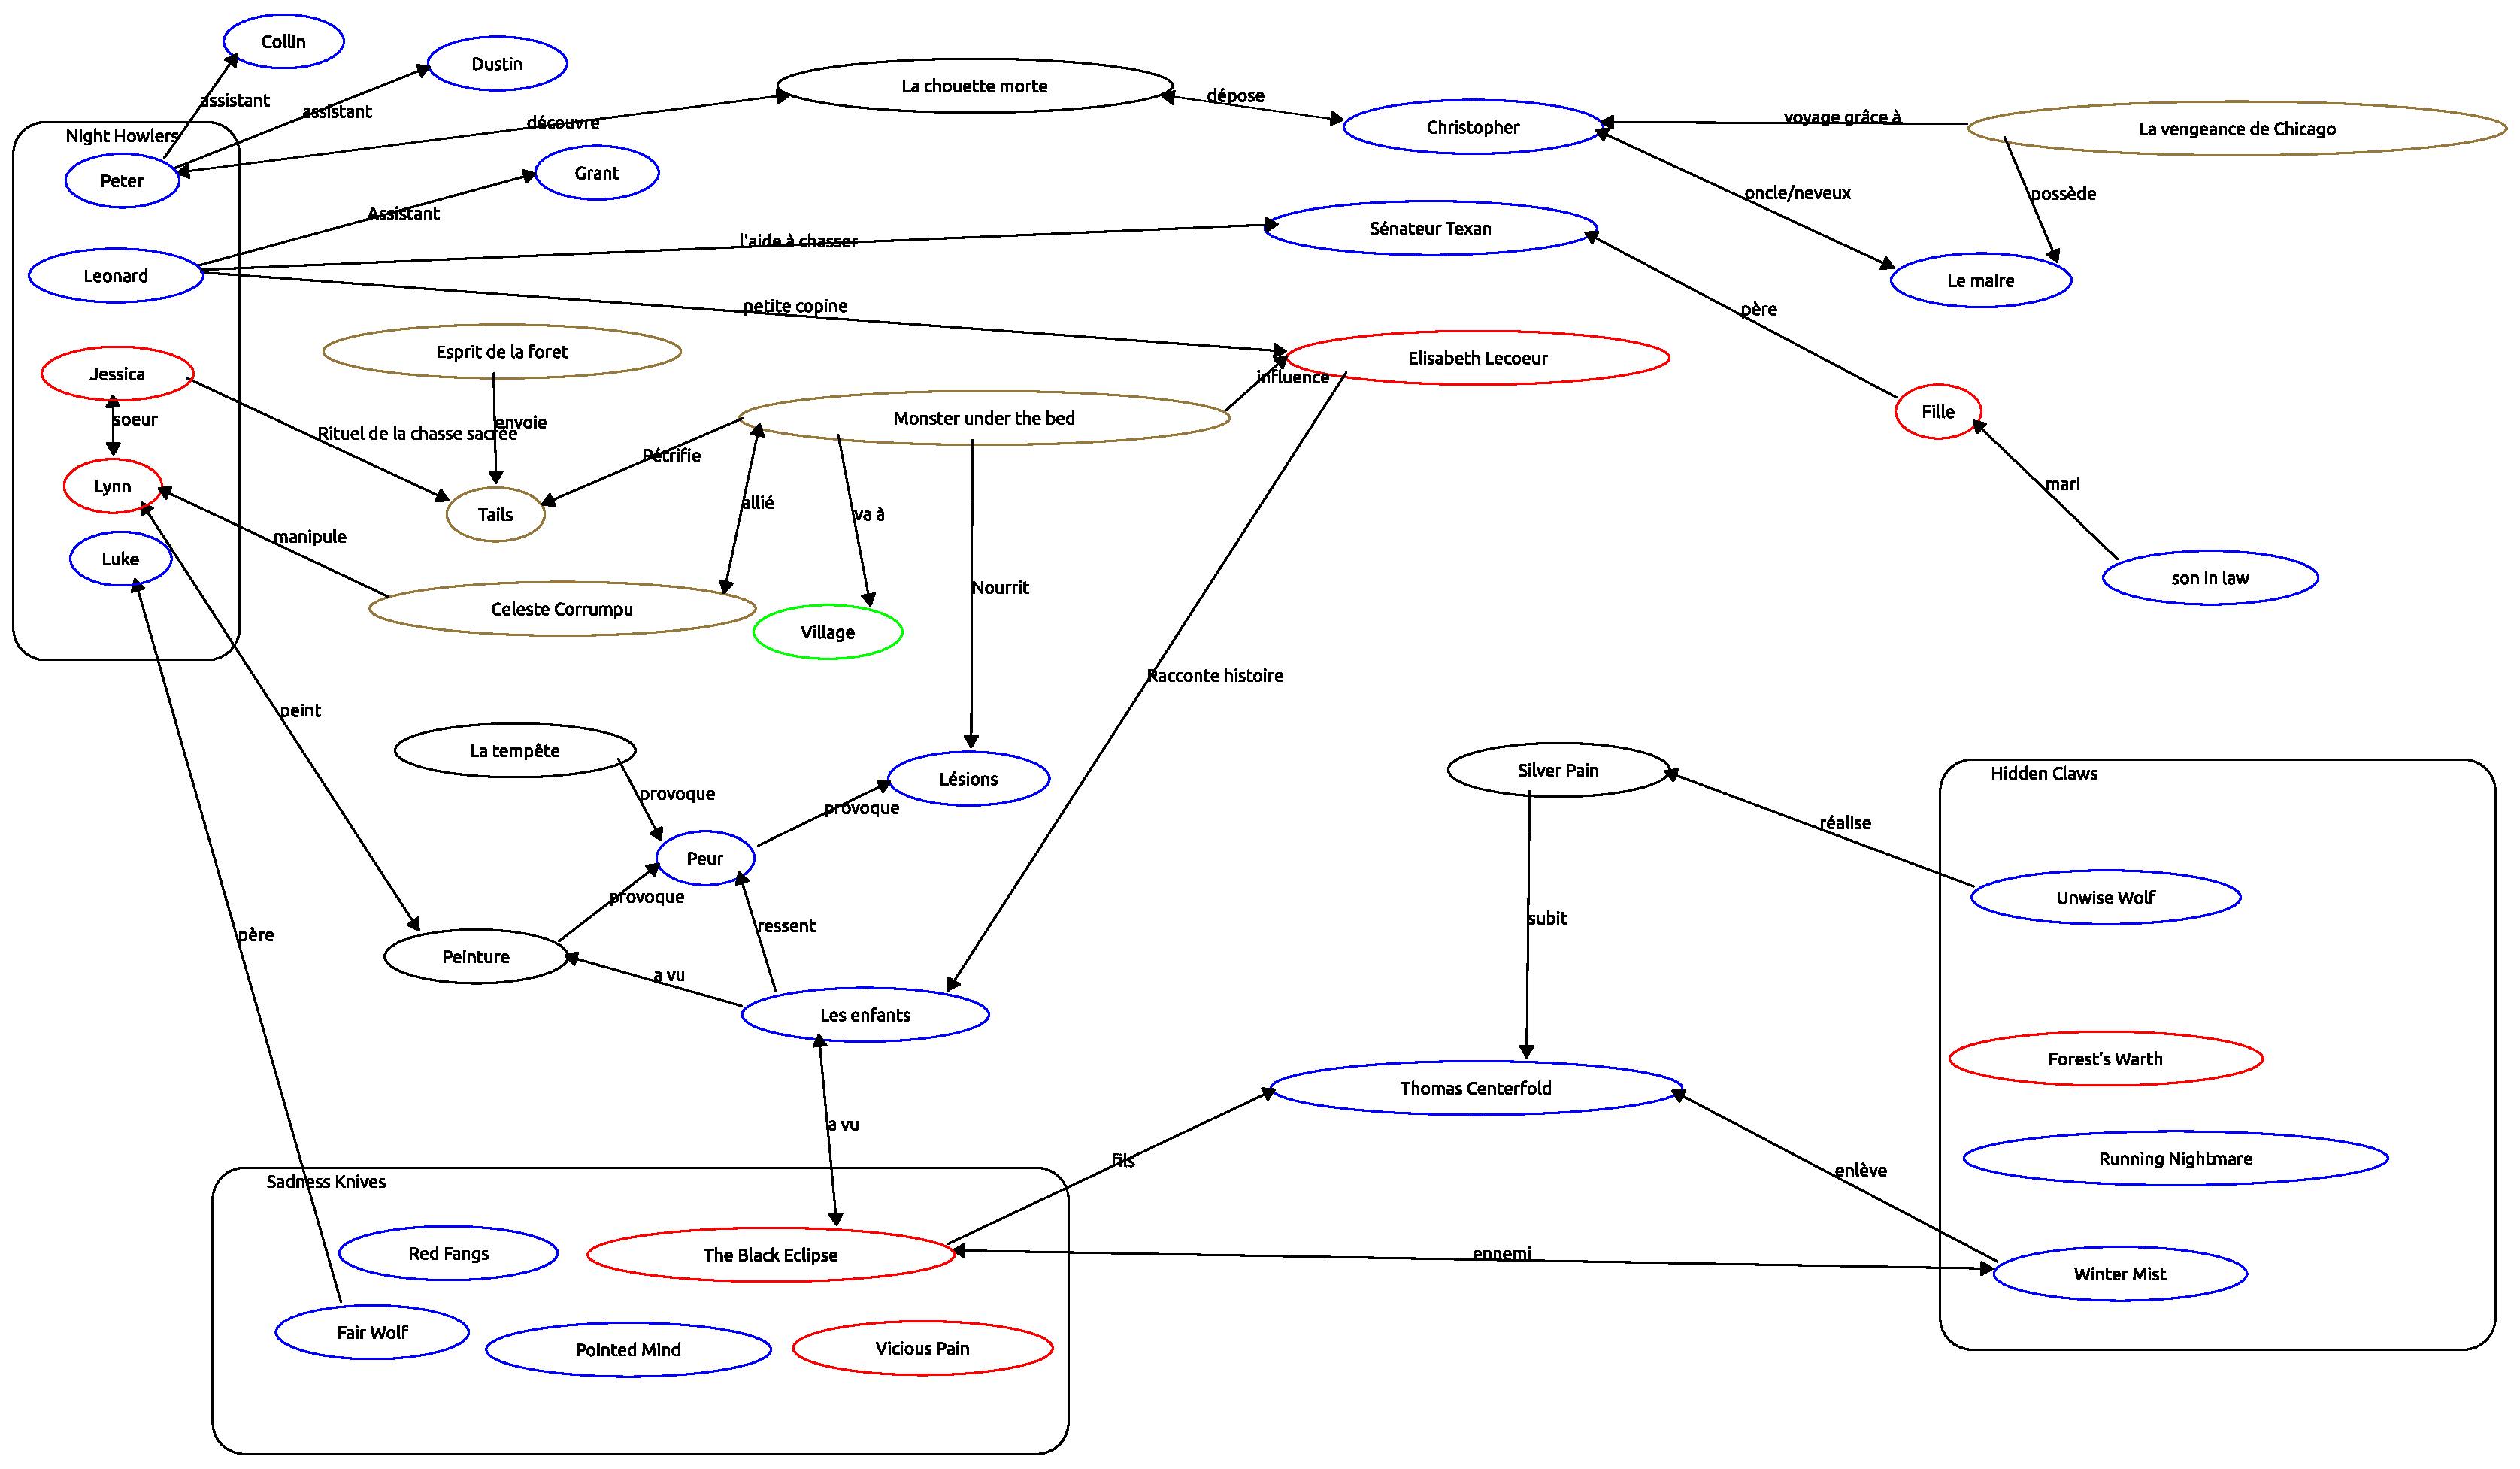
\includegraphics[width=\textwidth]{canada_2.eps}
\caption{Schéma du scénario définissant l'ensemble des relations entre les différents personnages. Image vectorielle, réaliser avec le logiciel \href{https://github.com/obiwankennedy/rmindmap}{Rmindmap}}
%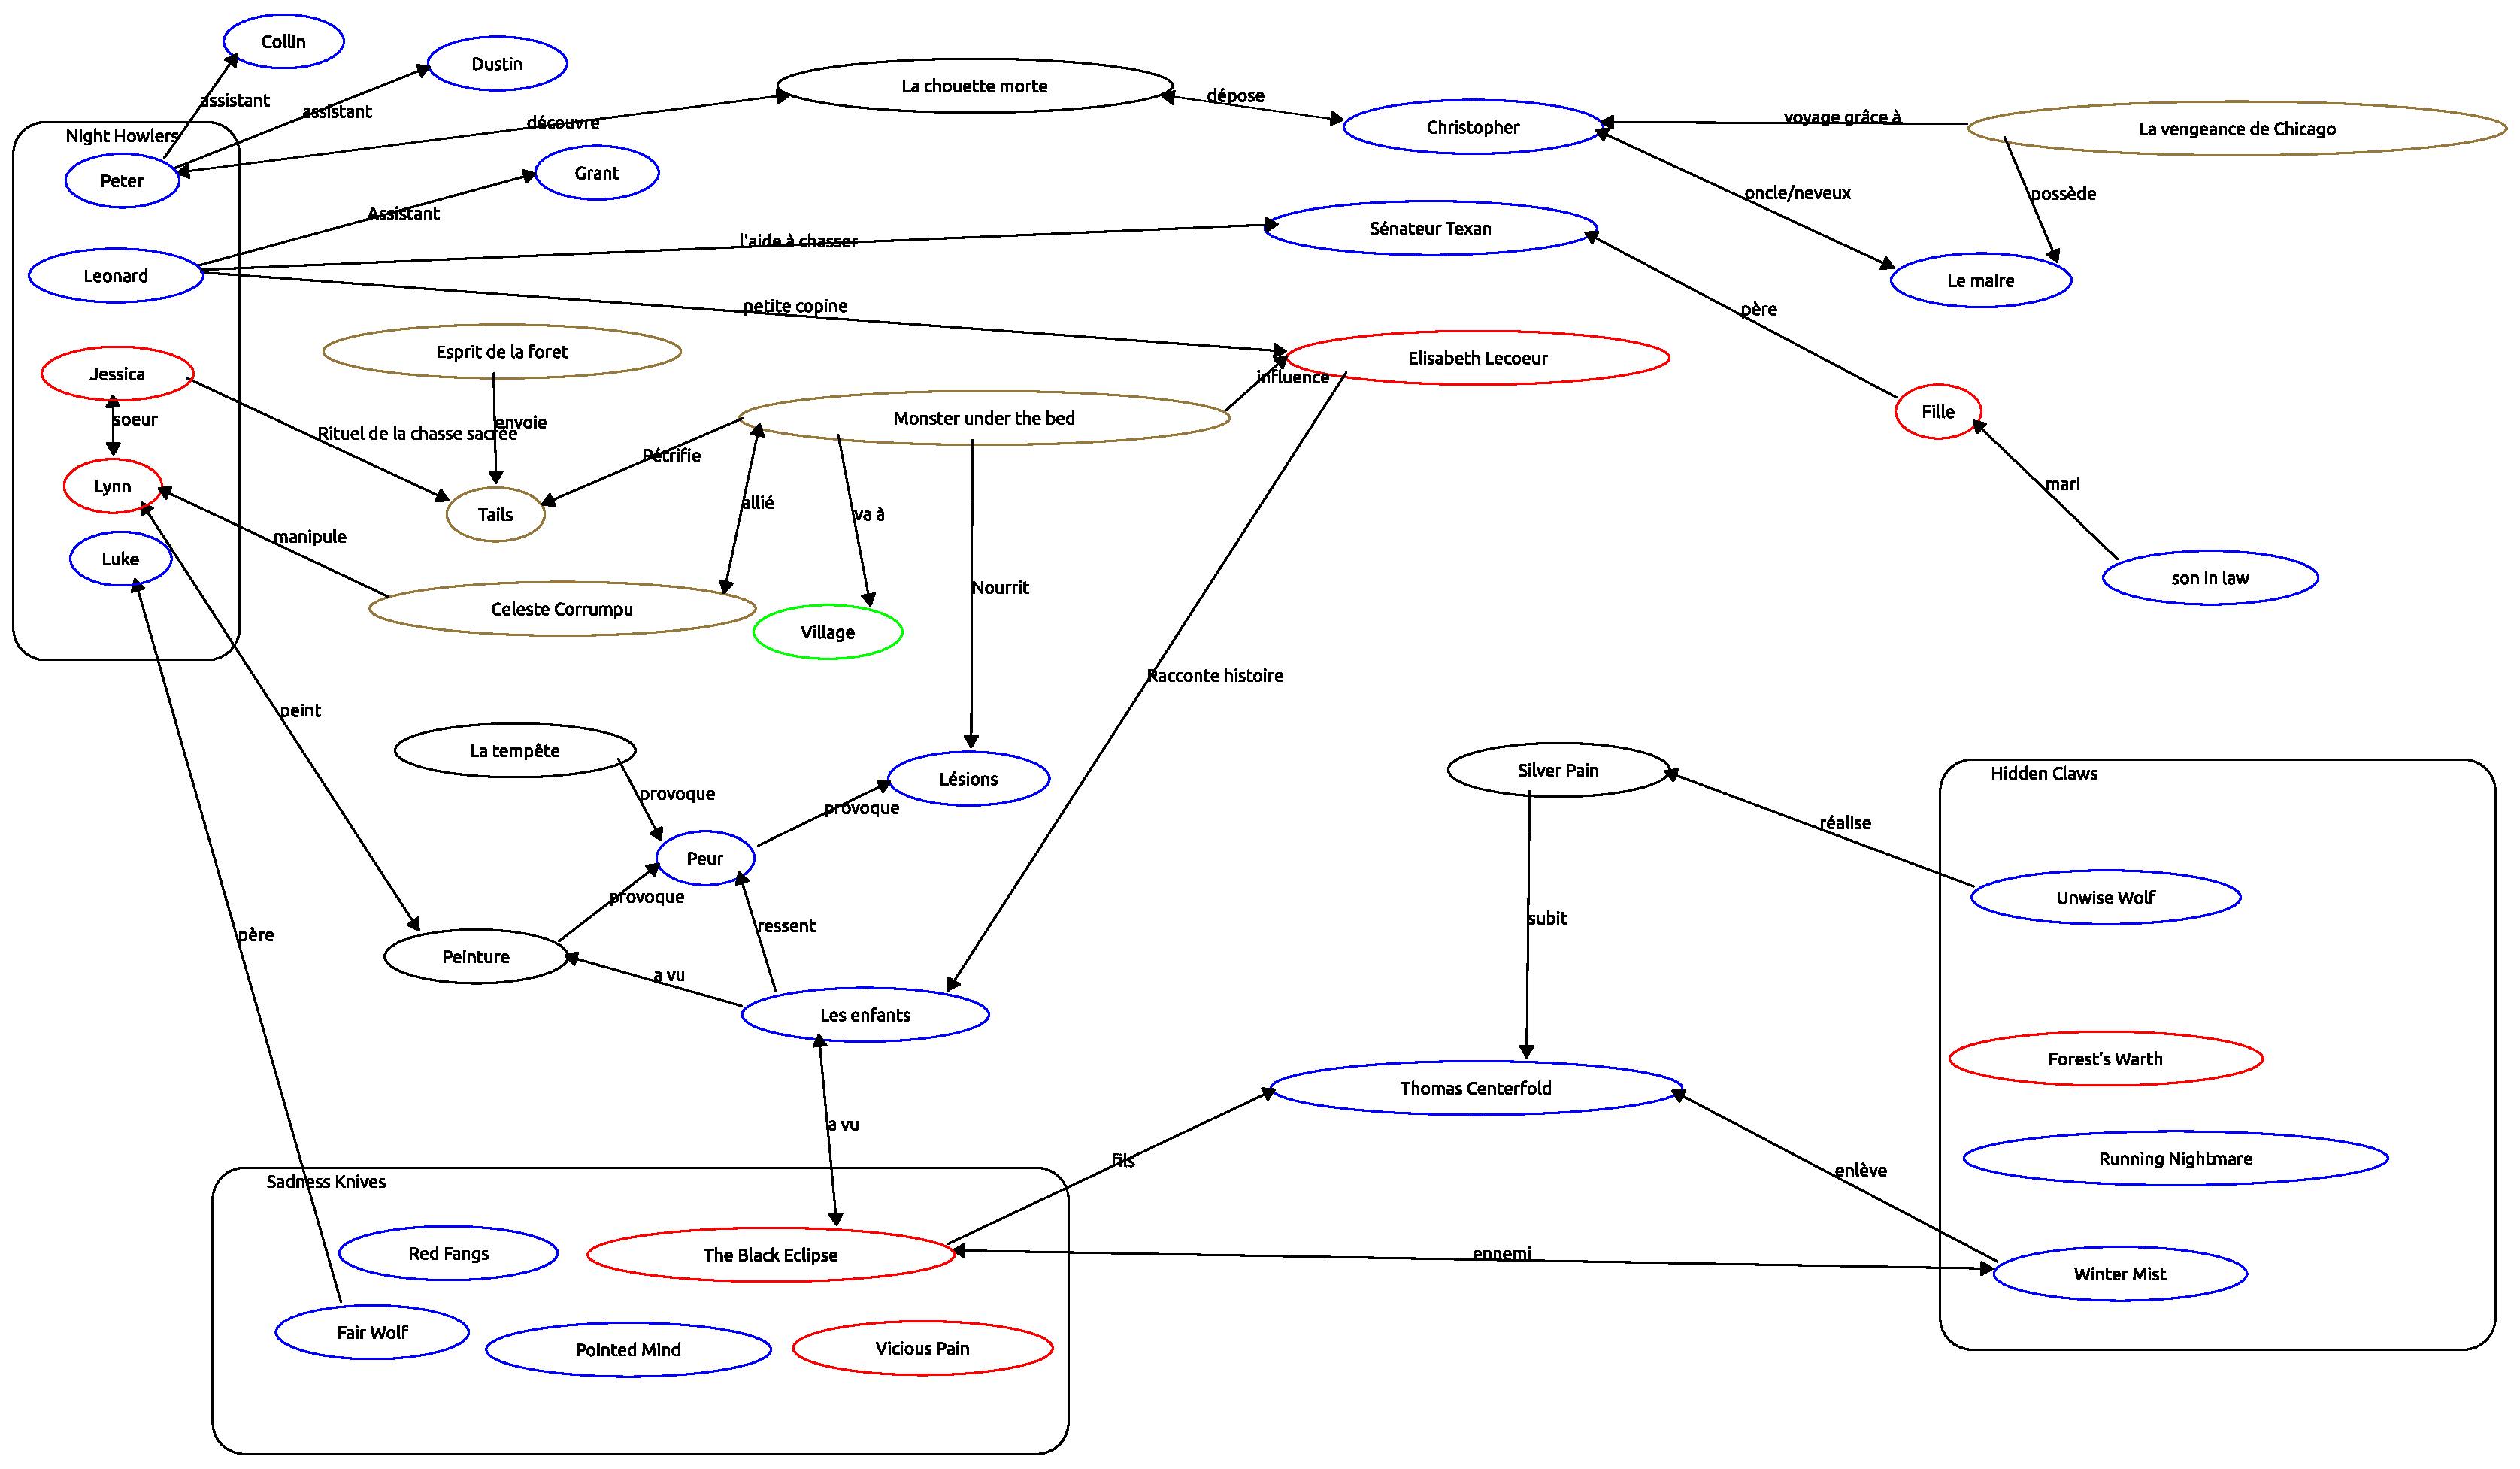
\includegraphics[width=\textwidth]{canada_2.eps}
\label{fig:mindmap}
\end{figure}

\end{flushleft}
\end{document}
